\documentclass[onecolumn,10pt]{jhwhw}

\usepackage{epsfig} %% for loading postscript figures
\usepackage{amsmath}
\usepackage{graphicx}
\usepackage{grffile}
\usepackage{pdfpages}
\usepackage{algpseudocode}
\usepackage{wrapfig}
\usepackage{pgfplots}
\usepackage{amsfonts}
\usepackage{booktabs}
\usepackage{siunitx}
\usepackage{commath}

% Default fixed font does not support bold face
\DeclareFixedFont{\ttb}{T1}{txtt}{bx}{n}{12} % for bold
\DeclareFixedFont{\ttm}{T1}{txtt}{m}{n}{12}  % for normal

% Custom colors
\usepackage{color}
\usepackage{listings}
\usepackage{framed}
\usepackage{caption}
\usepackage{bm}
\captionsetup[lstlisting]{font={small,tt}}

\definecolor{mygreen}{rgb}{0,0.6,0}
\definecolor{mygray}{rgb}{0.5,0.5,0.5}
\definecolor{mymauve}{rgb}{0.58,0,0.82}

\lstset{ %
  backgroundcolor=\color{white},   % choose the background color; you must add \usepackage{color} or \usepackage{xcolor}
  basicstyle=\ttfamily\footnotesize, % the size of the fonts that are used for the code
  breakatwhitespace=false,         % sets if automatic breaks should only happen at whitespace
  breaklines=true,                 % sets automatic line breaking
  captionpos=b,                    % sets the caption-position to bottom
  commentstyle=\color{mygreen},    % comment style
  deletekeywords={...},            % if you want to delete keywords from the given language
  escapeinside={\%*}{*)},          % if you want to add LaTeX within your code
  extendedchars=true,              % lets you use non-ASCII characters; for 8-bits encodings only, does not work with UTF-8
  frame=single,                    % adds a frame around the code
  keepspaces=true,                 % keeps spaces in text, useful for keeping indentation of code (possibly needs columns=flexible)
  columns=flexible,
  keywordstyle=\color{blue},       % keyword style
  language=Python,                 % the language of the code
  morekeywords={*,...},            % if you want to add more keywords to the set
  numbers=left,                    % where to put the line-numbers; possible values are (none, left, right)
  numbersep=5pt,                   % how far the line-numbers are from the code
  numberstyle=\tiny\color{mygray}, % the style that is used for the line-numbers
  rulecolor=\color{black},         % if not set, the frame-color may be changed on line-breaks within not-black text (e.g. comments (green here))
  showspaces=false,                % show spaces everywhere adding particular underscores; it overrides 'showstringspaces'
  showstringspaces=false,          % underline spaces within strings only
  showtabs=false,                  % show tabs within strings adding particular underscores
  stepnumber=1,                    % the step between two line-numbers. If it's 1, each line will be numbered
  stringstyle=\color{mymauve},     % string literal style
  tabsize=4,                       % sets default tabsize to 2 spaces
}

\author{John Karasinski}
\title{Extra Credit}

\begin{document}%
%\maketitle
%
% \begin{lstlisting}
% \end{lstlisting}
\noindent Choose one of the following:\\
\\
1. The Monty Hall Problem: If you're unfamiliar with this problem, please see the following video (http://www.youtube.com/watch?v=9vRUxbzJZ9Y).
I want you to write R syntax that will simulate this scenario, such that a person selects a choice of 1 in 3 doors (behind one of which is a prize), and is given the opportunity to switch their selection when given information about one of the remaining doors that does not contain the prize. Your syntax should show how often the person would win if they stayed with their original selection, and how often they will win if they switch their selection after seeing that one of the remaining doors is not a winner. As we're always interested in large number statistics, you should compare the winning frequency for either strategy (staying vs. switching) when a person is confronted with this situation once, 10 times, 100 times, 500 times, and 1,000 times in a row. Further, we should probably see what these outcomes look like at each number of trials 500 times (i.e., one trial outcomes 500 times, 10 trial outcomes 500 times, etc.). Once this is complete graph the average outcome for each trial size (one, 10, 100, etc.) with error bars; you should graph the outcomes for staying and switching for comparison.\\
\\
2. RPG Dice Simulator: As a nerd I like to get my RPG on, but I hate fussing over a dice pool. Simplify my life by creating a function that will allow me to specify the number of dice I want to use per roll, the number of faces on each die (assume all dice used in a role have the same number of faces), whether I will sum the scores of each die or will have a minimum value needed to count as a success per die (i.e., I need to role 6s using 6 10-sided die, each die with a score 6 or greater counts as a success and each die with a score of 5 or less counts as nothing), and whether I will include botches or not as an outcome for roles (i.e., when rolling for successes such as scores of 6 or greater per die, rolls of 1 count as a botch and deduct from the number of successes; if there are more botches than successes then the roll is botched). This way it doesn't matter if I'm rolling for damage in D\&D or for actions in White Wolf, I will always have a handy dice simulator.\\
Example scenarios the simulator should be able to handle: (1) I want to role 1d20 and I just want to know the score; (2) I want to roll 2d6 and I want to know my summed scores (e.g., 1d6 = 3 \& 1d6 = 5 for a score of 8); (3) I want to roll 4d10 where I need to roll 5s or greater such that each roll of 5 or greater counts as a success (e.g., 2d10 $<$ 5 and 2d10 $>=$ 5 for a score of 2 successes); (4) the same scenario as (3) but now each 1 rolled detracts from the number of successes (e.g., 1d10 = 1, 1 $<$ 1d10 $<$ 5, and 2d10 $>=$ 5 for a score of 1 success and 2d10 = 1, 1 $<$ 1d10 $<$ 5, and 1 d10 $>=$ 5 for a score of -1 successes; a botch). Once you have your function working, simulate the following dice roll scenarios and create figures depicting each.\\
\\
a. Roll 1d6 1,000 times, frequency of each outcome?\\
b. Roll 2d6 1,000 times, frequency of each outcome? Use the summed scores of each die as your outcome.\\
c. Roll 6d10 1,000 times, frequency of each outcome? Treat a score of 6 or better as a success and scores less than 6 as nothing, the outcome is total number of successes (include the frequency of no successes).\\
d. Same as (c) above except now scores of 1 count as a botch. Each botch is subtracted from each success. If there are more botches than success (i.e., -1 successes) then the overall outcome is a botch. Now depict the frequency of botching, and total number of successes (as before, include the frequency of no successes).\\
\\
Instructions:\\
Pick one project to complete.\\
The project should consist of a brief write-up introducing relevant theory behind each simulation problem, your simulation method, your results, and a summary of your conclusions. I'm looking for short papers ranging 5-8 pages in length. These papers should focus on the simulation methodology and results, with these sections making up the bulk of the paper.\\
**** Include all R code in Appendices so I can review it.\\
**** Hard copies due to me by the end of lecture on Thursday Dec. 3, 2015.\\
**** Grading will be based on completeness of answers, quality of reports, and both efficacy and efficiency of your code.\\
**** These projects should represent your own work (not online resources or other students). To clarify, online resources for functions, etc. is fine (and should be cited), but online searches for solutions to these specific problems (and the use of functions specific to these problems) is not.

% \begin{figure}[h!]
% \begin{center}
% 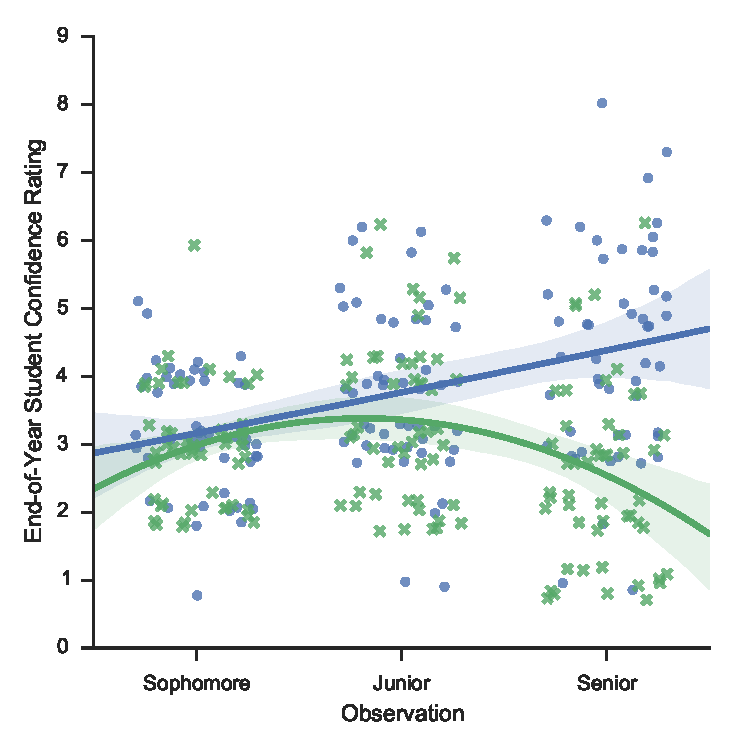
\includegraphics[width=1\textwidth]{prob5-quad.pdf}
% \label{fig:on}
% \end{center}
% \caption{Quadratic trajectories for end-of-year confidence ratings for students in public schools (green) and private schools (blue). Shaded regions represent 95\% confidence regions. (Some jitter introduced for visibility.)}
% \end{figure}

\end{document}
